\chapter{スピン幾何学と最初のもつれ状態}

\lectureoverview{もつれは部分を持つ系に属するが、二スピン問題を正直に読み解くには、まず一スピンの仕組みが完成していなければならない。そこでまず任意軸に沿ったスピンから始め、二つの方向の間の遷移確率を導き、測定をフィルターとして解釈し、可換性を両立する可観測量の基準として同定する。次に数え上げの議論により、二つのスピンは別々に用意された二つのスピンが供給できるよりも多くの純粋状態を持つことが明らかになる。余分な状態はもつれており、最も単純な例ですでに、各電子は個別には完全に無偏極でありながら、対の相関は確定している。}

\section{一スピン問題の完成}

ベルの定理は後回しでよい。もつれそのものは二つの電子から始まるが、一つの電子の残りの構造はあらゆる計算に入ってくる。したがって、二つのコピーを組み合わせる前に、二状態系を完成させよう。

通常の空間単位ベクトルを選ぶ
\begin{equation}
  \hat n=(n_1,n_2,n_3),
  \qquad
  n_1^2+n_2^2+n_3^2=1.
  \label{eq:l04-unit-pointer}
\end{equation}
ラベル\(1,2,3\)は\(x,y,z\)と呼んでも同じである。重要なのは、軸が一つの整合した右手座標系をなすことである。

\begin{classroomqa}
\lecturetimestamp{00:02:33}
\audiencequestion{黒板に描かれた座標三つ組は右手系か？}
\lecturerresponse{最初のスケッチは左手系である。第二軸を反転するか、二つの軸を整合的に付け替えれば修正される。以下の計算は固定された右手系の規約のみを用いる。スケッチの偶発的な向きに物理はない。}
\end{classroomqa}

スピンには三つの可観測な成分があり、パウリ行列で表される
\begin{equation}
  \begin{aligned}
    \sigma_1&=
    \begin{pmatrix}0&1\\1&0\end{pmatrix},
    &
    \sigma_2&=
    \begin{pmatrix}0&-i\\i&0\end{pmatrix},\\[0.5em]
    \sigma_3&=
    \begin{pmatrix}1&0\\0&-1\end{pmatrix}.
  \end{aligned}
\end{equation}
\(\hat n\)に沿った成分は、ポインターとこの行列値ベクトルとの通常の空間内ドット積である：
\begin{equation}
  \sigma_{\hat n}
  \equiv
  \boldsymbol{\sigma}\cdot\hat n
  =
  n_1\sigma_1+n_2\sigma_2+n_3\sigma_3.
  \label{eq:l04-sigma-dot-n}
\end{equation}
このドット積は物理的三次元空間におけるものである。二つの状態ベクトルの内積ではない。

\begin{figure}[htbp]
\centering
\includegraphics[width=0.82\linewidth]{lecture_04_figure_02.png}
\caption{\(\hat n\)に沿った空間成分は、三つの行列可観測量の線形結合になる。}
\lectureframe{00:05:09}
\end{figure}

パウリ行列を代入すると
\begin{equation}
  \sigma_{\hat n}
  =
  \begin{pmatrix}
    n_3 & n_1-in_2\\
    n_1+in_2 & -n_3
  \end{pmatrix}.
  \label{eq:l04-sigma-n-matrix}
\end{equation}
次のように略記すると便利である
\begin{equation}
  n_-=n_1-in_2,
  \qquad
  n_+=n_1+in_2=n_-^*,
\end{equation}
したがって
\begin{equation}
  \sigma_{\hat n}
  =
  \begin{pmatrix}
    n_3&n_-\\
    n_+&-n_3
  \end{pmatrix}.
\end{equation}
実数の対角成分と共役な非対角成分が、この演算子をエルミートにする。

\begin{figure}[htbp]
\centering
\includegraphics[width=0.84\linewidth]{lecture_04_figure_03.png}
\caption{任意軸スピン可観測量の明示的な二行二列形。}
\lectureframe{00:07:34}
\end{figure}

操作上、\(\sigma_{\hat n}\)を測定することは、強い磁場を\(\hat n\)に沿って向け、スピン依存の応答を観測することを意味し、講義では光子が放出されるかどうかで表される。行列と実験室での問いは、同じ測定の二つの記述である。

二つの小さな恒等式が残りの計算を担う。第一に、
\begin{equation}
  \sigma_{\hat n}^{\,2}=I.
  \label{eq:l04-sigma-n-square}
\end{equation}
これは式~\eqref{eq:l04-sigma-n-matrix}をそれ自身に掛けるか、
\begin{equation}
  \sigma_i^2=I,
  \qquad
  \sigma_i\sigma_j=-\sigma_j\sigma_i
  \quad(i\ne j).
\end{equation}
を用いることで従う。したがって\(\sigma_{\hat n}\)のすべての固有値\(\lambda\)は\(\lambda^2=1\)を満たし、可能な結果は
\begin{equation}
  \lambda=\pm1.
\end{equation}
のみである。第二に、
\begin{equation}
  n_+n_-
  =n_1^2+n_2^2
  =1-n_3^2
  =(1-n_3)(1+n_3).
  \label{eq:l04-nplus-nminus}
\end{equation}
これは深い定理ではないが、固有ベクトルの代数を制御下に保つ恒等式である。

\section{準備から確率へ}

電子を\(\hat n\)に沿ったスピン\(+1\)で準備し、次に異なる方向\(\hat m\)に沿って測定する。中心となる一スピンの問いは
\begin{equation}
  P(m,+\mid n,+)
  =
  P(\sigma_{\hat m}=+1\mid\sigma_{\hat n}=+1).
  \label{eq:l04-central-probability}
\end{equation}
対称性は、答えが\(\hat n\)と\(\hat m\)の間の角度のみに依存し、二つの方向を入れ替えても変わらないことを示唆する。これらの期待は有用な検査であって、確率の公準の代わりにはならない。

\begin{classroomqa}
\lecturetimestamp{00:14:03}
\audiencequestion{量子力学自体が三つのパウリ行列はスピン演算子であると教えるのか、それともそれは実験から学ぶのか？}
\lecturerresponse{この同定は量子力学の蓄積された経験的構造の一部であり、一つの孤立した実験の結果ではない。繰り返されるスピン実験は確率的規則性を明らかにし、行列形式はそれらの規則性を符号化するためにアインシュタイン、ボルン、ハイゼンベルク、ディラックらの仕事を通じて構築された。公準はデータによって制約された、極めて成功した推測である。}
\end{classroomqa}

とする
\begin{equation}
  \sigma_{\hat n}\ket{n,+}=\ket{n,+},
  \qquad
  \sigma_{\hat m}\ket{m,+}=\ket{m,+}.
  \label{eq:l04-nm-eigenstates}
\end{equation}
記号\(n,+\)と\(m,+\)はケットの内部のラベルである。それらは固有値が\(+1\)である固有状態を同定する。

\begin{figure}[htbp]
\centering
\includegraphics[width=0.76\linewidth]{lecture_04_figure_04.png}
\caption{\(\hat n\)と\(\hat m\)に沿ったスピンの\(+1\)固有状態。}
\lectureframe{00:17:36}
\end{figure}

最初に計算すべき対象は確率振幅
\begin{equation}
  \mathcal A(m,+\mid n,+)=\braket{m,+}{n,+}.
\end{equation}
確率はその絶対値の二乗である：
\begin{equation}
  P(m,+\mid n,+)
  =
  \left|\braket{m,+}{n,+}\right|^2.
  \label{eq:l04-born-nm}
\end{equation}
まず振幅、次に確率：この順序が本質的な量子の一歩である。

\begin{figure}[htbp]
\centering
\includegraphics[width=0.78\linewidth]{lecture_04_figure_05.png}
\caption{準備された\(n\)状態と測定される\(m\)状態の間の重なりが確率振幅である。}
\lectureframe{00:19:59}
\end{figure}

\subsection{固有状態を解く}

\(\sigma_{\hat n}\)の固有ベクトルの候補を\(+1\)として
\begin{equation}
  \begin{pmatrix}\alpha\\\beta\end{pmatrix}.
\end{equation}
と書く。規格化は後回しにしてよく、全体の位相は物理的効果を持たない。したがって南極の座標パッチから離れて、\(\alpha=1\)と選び、\(\beta=z\)と書いてよい。
\begin{equation}
  \begin{pmatrix}
    n_3&n_-\\
    n_+&-n_3
  \end{pmatrix}
  \begin{pmatrix}1\\z\end{pmatrix}
  =
  \begin{pmatrix}1\\z\end{pmatrix}
\end{equation}
の上成分は
\begin{equation}
  n_3+n_-z=1,
  \qquad
  z=\frac{1-n_3}{n_-}.
  \label{eq:l04-z-solution}
\end{equation}
を与える。下成分は、式~\eqref{eq:l04-nplus-nminus}を用いれば同じ条件を与える。

規格化されていないベクトルのノルムの二乗は
\begin{align}
  \begin{pmatrix}
    1&\dfrac{1-n_3}{n_+}
  \end{pmatrix}
  \begin{pmatrix}
    1\\[3pt]\dfrac{1-n_3}{n_-}
  \end{pmatrix}
  &=
  1+\frac{(1-n_3)^2}{n_+n_-}
  \notag\\
  &=
  1+\frac{1-n_3}{1+n_3}
  =
  \frac{2}{1+n_3}.
  \label{eq:l04-unnormalized-norm}
\end{align}
である。したがって規格化された選択は
\begin{equation}
  \ket{n,+}
  =
  \sqrt{\frac{1+n_3}{2}}
  \begin{pmatrix}
    1\\[5pt]\dfrac{1-n_3}{n_-}
  \end{pmatrix}.
  \label{eq:l04-normalized-n-state}
\end{equation}
となる。\(n_3=-1\)では、状態自体は特異でないにもかかわらず、この座標表示は特異になる。固有状態は単に\(\ket d=(0,1)^T\)である。特異性は位相の取り方に属するものであり、スピンに属するものではない。

\(n\)を\(m\)に置き換えて複素共役をとると
\begin{equation}
  \bra{m,+}
  =
  \sqrt{\frac{1+m_3}{2}}
  \begin{pmatrix}
    1&
    \dfrac{1-m_3}{m_+}
  \end{pmatrix}.
\end{equation}
が得られる。この内積は不快に見え、その共役を掛けるとさらに悪く見える。式~\eqref{eq:l04-nplus-nminus}を繰り返し用いると、結果は
\begin{equation}
  \begin{aligned}
    P(m,+\mid n,+)
    &=\frac{1+n_1m_1+n_2m_2+n_3m_3}{2}\\
    &=\frac{1+\hat n\cdot\hat m}{2}.
  \end{aligned}
  \label{eq:l04-spin-transition-probability}
\end{equation}
に簡約される。\(\theta_{nm}\)を二つの空間方向のなす角とすれば、
\begin{equation}
  P(m,+\mid n,+)
  =
  \frac{1+\cos\theta_{nm}}{2}
  =
  \cos^2\frac{\theta_{nm}}{2}.
  \label{eq:l04-half-angle-probability}
\end{equation}

\begin{classroomqa}
\lecturetimestamp{00:32:47}
\audiencequestion{二つの状態が直交するのだから、内積は消えなければならないのか。}
\lecturerresponse{いいえ。ラベル\(m,+\)と\(n,+\)は、一つの固定された観測量の異なる固有値ではなく、異なる測定軸を指している。\(m=n\)ならば、二つの状態は一致し、それらの内積は1である。それらが直交するのは、物理的な方向が反対であり、一方の状態が同じスピン成分の\(+1\)状態で他方が\(-1\)状態となるときだけである。}
\end{classroomqa}

\section{確率公式の意味するもの}

式~\eqref{eq:l04-spin-transition-probability}は三つの即座の検査を通過する：
\begin{align}
  \hat m=\hat n
  &\quad\Longrightarrow\quad P=1,
  \notag\\
  \hat m=-\hat n
  &\quad\Longrightarrow\quad P=0,
  \notag\\
  \hat m\cdot\hat n=0
  &\quad\Longrightarrow\quad P=\frac12.
\end{align}
答えは相対角のみに依存し、\(m\leftrightarrow n\)の下で対称である。装置全体を回転させても予測は変わらない。

これがスピン1/2が行う驚くべき妥協である。どの軸に沿っても、観測結果は\(+1\)または\(-1\)のままであり、分数のスピン値になることは決してない。滑らかな回転依存性は、代わりにこれら二つの離散的な答えの確率に現れる。

\begin{classroomqa}
\lecturetimestamp{00:39:20}
\audiencequestion{繰り返しの試行が同じ電子に関するものだと、どうして分かるのか。また、確率はどのように測定されるのか。}
\lecturerresponse{一つの電子を空洞に閉じ込め、その電束を通して保存電荷を監視し、その電子を\(\hat n\)に沿って再準備し、\(\hat m\)に沿った測定を繰り返せばよい。同様に、多数の電子を同一に準備し、それぞれを一度ずつ測定してもよい。プラスとマイナスの結果の長期的な比は、統計誤差の範囲内で、どちらの手順でも同じである。}
\end{classroomqa}

\begin{classroomqa}
\lecturetimestamp{00:41:29}
\audiencequestion{アンサンブルの全成員を一つの集団的実験で測定しなければならないのか。}
\lecturerresponse{いいえ。各成員は同じプロトコルで準備され、別々に測定される。百万回のそのような試行が一つの統計的実験をなすのは、それらの結果の頻度が同じ確率を推定するという意味においてのみである。}
\end{classroomqa}

\begin{classroomqa}
\lecturetimestamp{00:42:23}
\audiencequestion{一つの電子を再利用するなら、それは何個の光子を放出できるのか。}
\lecturerresponse{固定された寿命の割り当てはない。各サイクルには、磁場を入れるときの外部仕事が含まれる。スピンがより高いエネルギーの向きにあるなら、その供給されたエネルギーは緩和の際に光子として出て行くことができる。したがって装置は、原理的には準備と放出のサイクルを無限に繰り返すことができる。}
\end{classroomqa}

回転不変性が分かった後なら、この公式は非常に速く得られる。\(\hat n\)を第三軸として選べば\(\ket{n,+}=(1,0)^T\)となり、\(\ket{m,+}\)の上成分から確率を読み取ればよい。しかし、その近道を最初から使うことは、今まさに明示的な計算が示した対称性を仮定することになる。

\begin{classroomqa}
\lecturetimestamp{00:43:33}
\audiencequestion{より良い基底の選択によって、醜い任意軸の固有ベクトルを取り除くことはできないか。}
\lecturerresponse{はい。回転とユニタリ変換が利用できるようになれば、座標軸を一方の方向に合わせて計算を短くできる。この段階では、明示的な計算は一つの目的を果たす。すなわち、選んだパウリ行列が本当に回転不変な答えを与えることを、その事実を仮定するのではなく検証するのである。}
\end{classroomqa}

\begin{classroomqa}
\lecturetimestamp{00:48:30}
\audiencequestion{答えが角度のみに依存する物理的な理由は何か。}
\lecturerresponse{構造的な答えは対称性の量子論に属する。空間回転は、スピン状態と観測量に作用するユニタリ変換によって表現される。その言語は後で登場する。今のところ、角度依存性はパウリ行列の計算によって獲得された結果である。}
\end{classroomqa}

\section{測定はフィルターである}

測定は単に数値を報告するだけではない。\(\sigma_{\hat m}\) を測定し、その結果が \(+1\) であれば、電子は \(\ket{m,+}\) に残される。装置は検出器と状態準備器の両方として働いたのであり、ちょうど偏光子が光子を検査し、透過した光子を自身の軸に沿った偏光状態に残すのとよく似ている。

この状態変化の規則により、同時測定の問題が具体的になる。二つの可観測量がともに再現可能な確定値をもちうるのは、両方の固有ベクトルであるような状態が存在する場合に限られる。

\begin{classroomqa}
\lecturetimestamp{00:51:29}
\audiencequestion{\(\sigma_1\) や \(\sigma_2\) のような二つの異なるスピン成分を同時に一つの測定で決定できるだろうか。}
\lecturerresponse{できない。それらの固有ベクトルは異なる。一方の成分の測定は電子をその成分の固有状態に残すが、その状態は他方の固有状態ではない。したがって最初の測定は、二番目の測定が要求する確定性を破壊する。}
\end{classroomqa}

一般の有限次元の場合の主張は、エルミート演算子について最も明快に述べられる。

\begin{theorem}
二つのエルミート演算子 \(A\) と \(B\) が同時対角化可能であるのは、それらが可換である場合に限る：
\begin{equation}
  [A,B]\equiv AB-BA=0.
  \label{eq:l04-commutator}
\end{equation}
同値な言い方をすれば、それらは完全な共通の正規直交固有基底をもつ。\end{theorem}

易しい向きについては、完全な基底に対して
\begin{equation}
  A\ket{\alpha_i}=\lambda_i\ket{\alpha_i},
  \qquad
  B\ket{\alpha_i}=\mu_i\ket{\alpha_i}
\end{equation}
が成り立つと仮定する。このとき
\begin{align}
  AB\ket{\alpha_i}
  &=\lambda_i\mu_i\ket{\alpha_i},
  \notag\\
  BA\ket{\alpha_i}
  &=\mu_i\lambda_i\ket{\alpha_i},
\end{align}
となるので、\(AB\) と \(BA\) はすべての基底ベクトル上で一致する。したがって \(AB=BA\) である。逆に、エルミート演算子 \(A\) と \(B\) が可換ならば、\(B\) は \(A\) の各固有空間を保つ。任意の縮退固有空間内で \(B\) を対角化すれば、共通の固有基底が得られる。

\begin{figure}[htbp]
\centering
\includegraphics[width=0.76\linewidth]{lecture_04_figure_06.png}
\caption{二つの可観測量は同じ固有ベクトルをもちながら、それらに異なる固有値を割り当てることがある。}
\lectureframe{00:55:45}
\end{figure}

\begin{classroomqa}
\lecturetimestamp{00:53:56}
\audiencequestion{\(x\) と \(y\) に沿って磁場を同時に印加し、それを同時測定と呼ぶことはできるだろうか。}
\lecturerresponse{磁場は一つの合成方向に足し合わされる。すると装置は \(\sigma_x\) と \(\sigma_y\) を別々に測定するのではなく、おそらく \(45^\circ\) にあるその合成軸に沿ったスピンを測定する。この試みられた構成は、二つの両立する読みではなく、第三の可観測量を生み出す。}
\end{classroomqa}

\section{すべての純粋な一スピン状態は一つの軸をもつ}

ここで固有ベクトル問題を逆にする。任意の規格化されたスピノル
\begin{equation}
  \ket\psi=
  \begin{pmatrix}\alpha\\\beta\end{pmatrix},
  \qquad
  |\alpha|^2+|\beta|^2=1,
  \label{eq:l04-general-spinor}
\end{equation}
が与えられたとき、
\begin{equation}
  \sigma_{\hat n}\ket\psi=\ket\psi?
  \label{eq:l04-reverse-eigenproblem}
\end{equation}
を満たす空間方向 \(\hat n\) は存在するだろうか。
存在する。講義ではまず数え上げによってその理由を見る。二つの複素成分は四つの実数を含む。規格化により一つが除かれ、物理的に無意味な全体位相によりさらに一つが除かれ、二つが残る。単位ポインタもまた、経度と緯度のような二つの独立な実パラメータをもつ。

\begin{classroomqa}
\lecturetimestamp{01:03:52}
\audiencequestion{\(\alpha\) と \(\beta\) がともに複素数であるのに、なぜ状態は二つの自由度しかもたないのか。}
\lecturerresponse{それらは四つの実成分から出発する。規格化条件が一つの実自由度を除き、状態全体に \(e^{i\theta}\) を掛けても確率は変わらないので、共通位相がさらに一つを除く。物理的に意味のある二つのパラメータが残り、単位ポインタの二つの角度と一致する。}
\end{classroomqa}

\begin{classroomqa}
\lecturetimestamp{01:04:20}
\audiencequestion{固有値も解く必要があるだろうか。}
\lecturerresponse{ここでは目標とする固有値は \(+1\) に固定されている。与えられたスピノルを上状態とする方向だけを探している。反対のポインタは、固有値 \(-1\) をもつ下状態として同じ射線を記述することになる。}
\end{classroomqa}

この数え上げは、対応関係が存在すべき理由を説明する。直接的な構成がそれを確認する。
\begin{align}
  n_1&=\bra\psi\sigma_1\ket\psi
      =2\operatorname{Re}(\alpha^*\beta),
  \notag\\
  n_2&=\bra\psi\sigma_2\ket\psi
      =2\operatorname{Im}(\alpha^*\beta),
  \notag\\
  n_3&=\bra\psi\sigma_3\ket\psi
      =|\alpha|^2-|\beta|^2.
  \label{eq:l04-bloch-components}
\end{align}
と定義する。規格化により \(n_1^2+n_2^2+n_3^2=1\) が得られ、直接代入すると式~\eqref{eq:l04-reverse-eigenproblem}が得られる。したがってすべての純粋な一スピン状態は、ある一つの空間軸に沿ったスピン上状態である。

この主張には操作的な版がある。同じ未知の純粋状態の多数のコピーを準備する。試行方向に沿ってバッチごとに測定し、磁石を調整し、すべての結果が上となる方向を探す。有限のデータでは方向は不確かさの範囲内でしか定まらないが、理想的な状態は一つの正確な軸をもつ。

問いはこの方法の一部であり、それを妨げるものではない。短い教室での余談が、十歳の子供たちが弦理論、余剰次元、そして周囲の中性子が頭痛を引き起こすかどうかについて自由に質問していたことを思い出させる。問いの細部は誤っているかもしれないが、混乱の要点をさらけ出す意欲は依然として価値がある。

\section{二つのスピンと局所演算子}

二つのスピンを組み合わせる前に、パウリ行列が \(\sigma_3\) 基底にどのように作用するかを記録しておく：
\begin{align}
  \sigma_1\ket u&=\ket d,
  &
  \sigma_1\ket d&=\ket u,
  \notag\\
  \sigma_2\ket u&=i\ket d,
  &
  \sigma_2\ket d&=-i\ket u,
  \notag\\
  \sigma_3\ket u&=\ket u,
  &
  \sigma_3\ket d&=-\ket d.
  \label{eq:l04-pauli-action-table}
\end{align}

\begin{figure}[htbp]
\centering
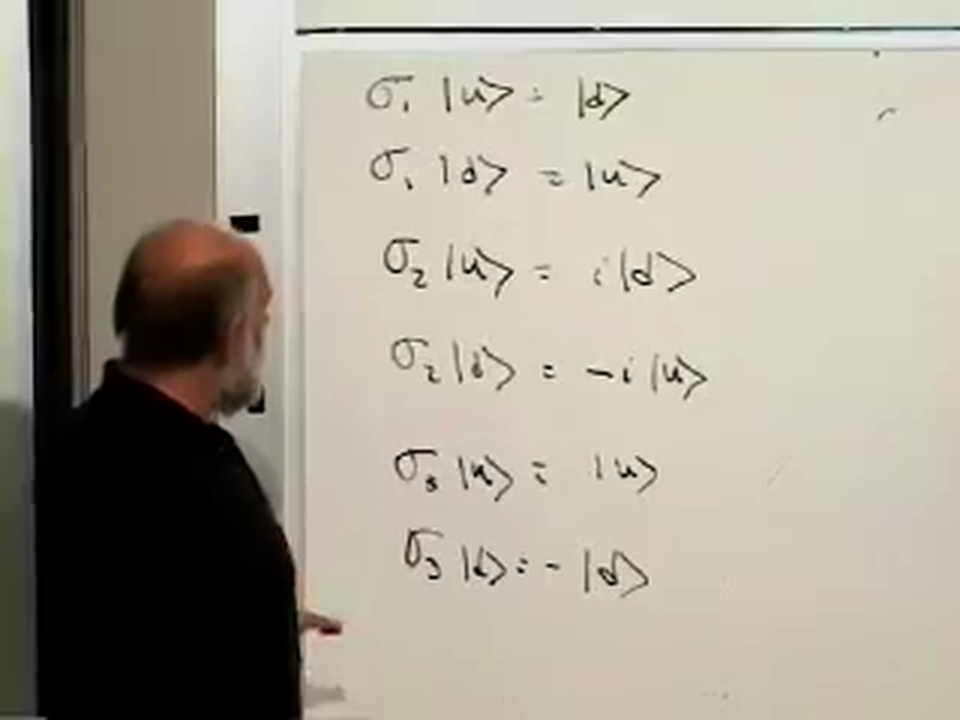
\includegraphics[width=0.80\linewidth]{lecture_04_figure_07.png}
\caption{パウリ作用表は、行列を上／下基底に関する規則としてまとめ直したものである。}
\lectureframe{01:09:35}
\end{figure}

ここで、位置が区別できるように保たれた二つの電子を考え、そのスピンだけが変化するとしよう。四つの基底状態は
\begin{equation}
  \ket{uu},
  \qquad
  \ket{du},
  \qquad
  \ket{ud},
  \qquad
  \ket{dd}.
  \label{eq:l04-two-spin-basis}
\end{equation}
である。最初のラベルは電子\(1\)に属し、二番目のラベルは電子\(2\)に属する。これらは、二つの第三成分測定の異なる結合結果を表すため、互いに正規直交である。

\begin{figure}[htbp]
\centering
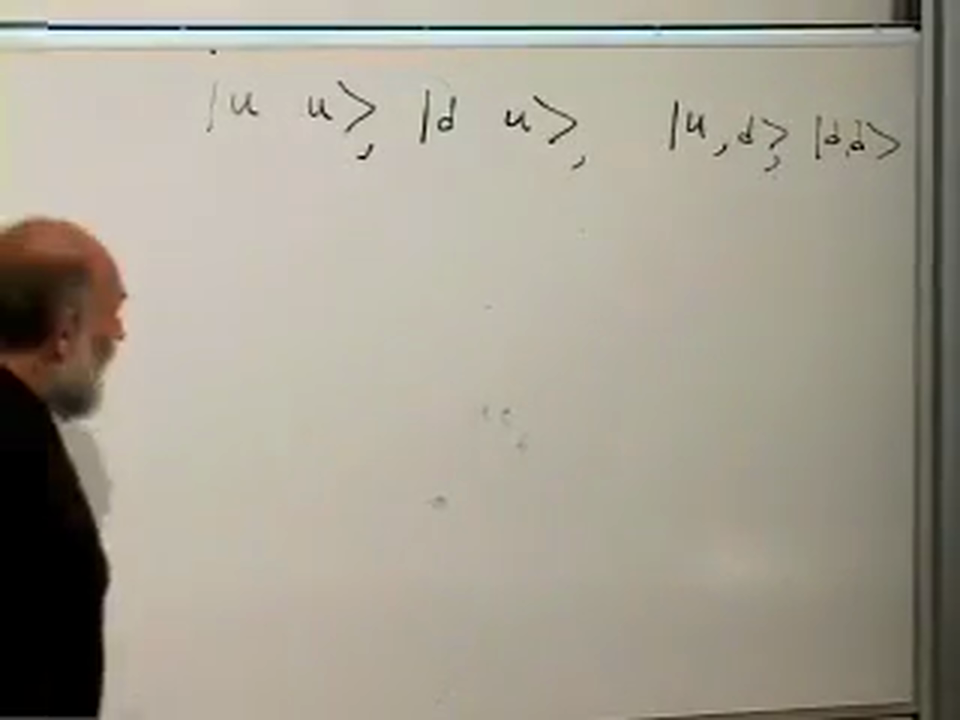
\includegraphics[width=0.82\linewidth]{lecture_04_figure_08.png}
\caption{4つの積基底ラベルは2スピン状態空間を張る。}
\lectureframe{01:11:40}
\end{figure}

電子\(1\)に作用する演算子を\(\sigma_i\)、電子\(2\)に作用する演算子を\(\tau_i\)と呼ぶ。より明示的には、
\begin{equation}
  \sigma_i\equiv\sigma_i\otimes I,
  \qquad
  \tau_i\equiv I\otimes\sigma_i.
\end{equation}
である。第一の組は第一のラベルにのみ作用し、第二の組は第二のラベルにのみ作用する：
\begin{align}
  \sigma_1\ket{ud}&=\ket{dd},
  &
  \sigma_1\ket{dd}&=\ket{ud},
  \notag\\
  \sigma_3\ket{dd}&=-\ket{dd},
  &
  \tau_2\ket{ud}&=-i\ket{uu}.
  \label{eq:l04-local-operator-examples}
\end{align}
演算子の四つの基底状態への作用が分かれば、線形性により、あらゆる二スピン状態への作用が定まる。

\begin{classroomqa}
\lecturetimestamp{01:17:47}
\audiencequestion{なぜ因子\(-i\)はケットの外に書かれるのか。それは両方の電子に作用するのか。}
\lecturerresponse{ケットの内側の記号は基底配置のラベルである。複素スカラーは状態ベクトル全体に掛かるため、標準的な記法ではそれを外側に置く。ここでのその起源は、\(\tau_2\)の第二のラベルへの作用であり、外側に書くことは、別個の物理的操作が両方の電子に施されたことを意味しない。}
\end{classroomqa}

\begin{classroomqa}
\lecturetimestamp{01:19:44}
\audiencequestion{\(i\)による掛け算は、通常空間における電子の回転を表すのか。}
\lecturerresponse{それ自体ではそうではない。それは状態空間における複素スカラー倍である。空間回転は後に特定のユニタリ演算子によって表される。この作用表における孤立した因子\(i\)は、文字通りの実空間の回転ではない。}
\end{classroomqa}

\section{4つではなく6つのパラメータ}

この対の一般的な純粋状態は
\begin{equation}
  \ket\Psi
  =
  c_{uu}\ket{uu}
  +c_{du}\ket{du}
  +c_{ud}\ket{ud}
  +c_{dd}\ket{dd}.
  \label{eq:l04-general-two-spin-state}
\end{equation}
である。4つの複素係数は8つの実数を与える。規格化が1つを除き、全体位相が1つを除く：
\begin{equation}
  8-1-1=6.
  \label{eq:l04-two-spin-parameter-count}
\end{equation}
別々に準備された電子\(1\)の純粋状態には2つの実パラメータが必要であり、電子\(2\)にはさらに2つ必要で、合計わずか4つである。欠けている2つのパラメータは計算間違いではない。それらは、各部分に別々の純粋状態を割り当てることができない対の純粋状態を示している。

まず、別々の準備から生じる状態を特定する。もし
\begin{equation}
  \ket{\psi_1}=\alpha_1\ket u+\beta_1\ket d,
  \qquad
  \ket{\psi_2}=\alpha_2\ket u+\beta_2\ket d,
\end{equation}
ならば
\begin{align}
  \ket{\psi_1}\otimes\ket{\psi_2}
  &=
  \alpha_1\alpha_2\ket{uu}
  +\alpha_1\beta_2\ket{ud}
  \notag\\
  &\quad
  +\beta_1\alpha_2\ket{du}
  +\beta_1\beta_2\ket{dd}.
  \label{eq:l04-product-expansion}
\end{align}
である。これは\emph{積状態}である。各電子は、2つの磁気的準備が独立に行われた場合と同様に、それ自身の偏極軸を持つ。

\begin{figure}[htbp]
\centering
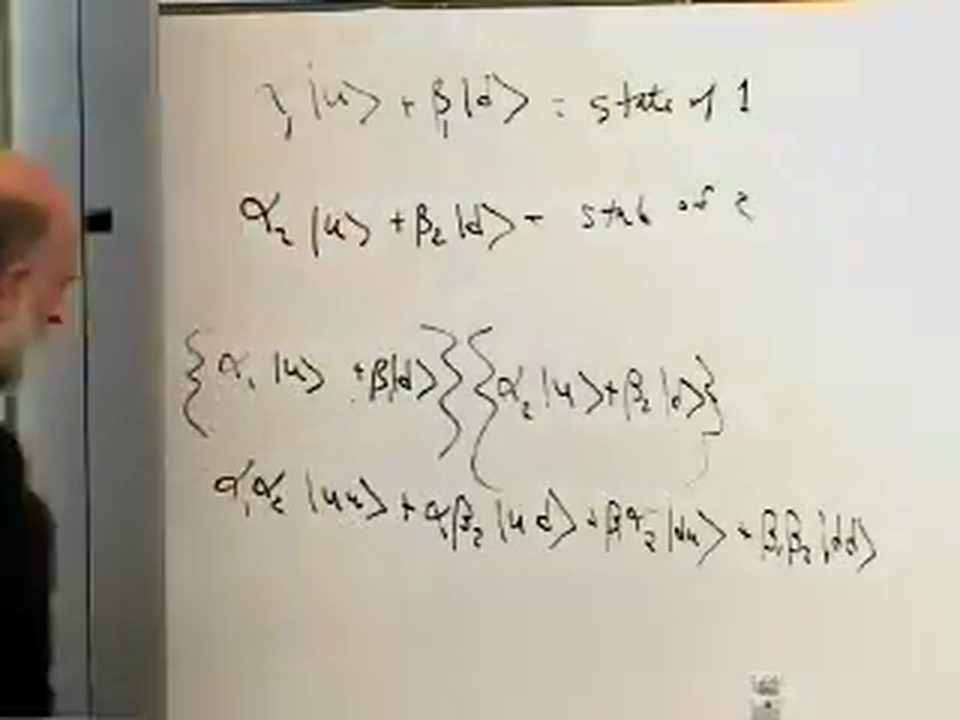
\includegraphics[width=0.84\linewidth]{lecture_04_figure_09.png}
\caption{2つの1スピン状態を掛けると、制限された4項の積状態が得られる。}
\lectureframe{01:25:15}
\end{figure}

4つの係数が
\begin{equation}
  C=
  \begin{pmatrix}
    c_{uu}&c_{ud}\\
    c_{du}&c_{dd}
  \end{pmatrix},
\end{equation}
のように並べられるとき、状態が積であるのは、\(C\)が階数1をもつ場合、すなわち
\begin{equation}
  c_{uu}c_{dd}-c_{ud}c_{du}=0.
  \label{eq:l04-product-condition}
\end{equation}
のときに限る。4つの振幅のほとんどの選択はこの条件を満たさない。それらはもつれている。

\section{最初のもつれ状態}

講義の最初の例は
\begin{equation}
  \ket{\psi_+}
  =
  \frac{1}{\sqrt2}
  \left(\ket{ud}+\ket{du}\right).
  \label{eq:l04-psi-plus}
\end{equation}
である。これは電子\(1\)の状態と電子\(2\)の状態とに因数分解できない。第三軸の測定で電子\(2\)が下向きと見出されれば、電子\(1\)は上向きである。電子\(2\)が上向きと見出されれば、電子\(1\)は下向きである。この対は、どちらの粒子も単独では持たない確定した情報を持つ。

\begin{figure}[htbp]
\centering
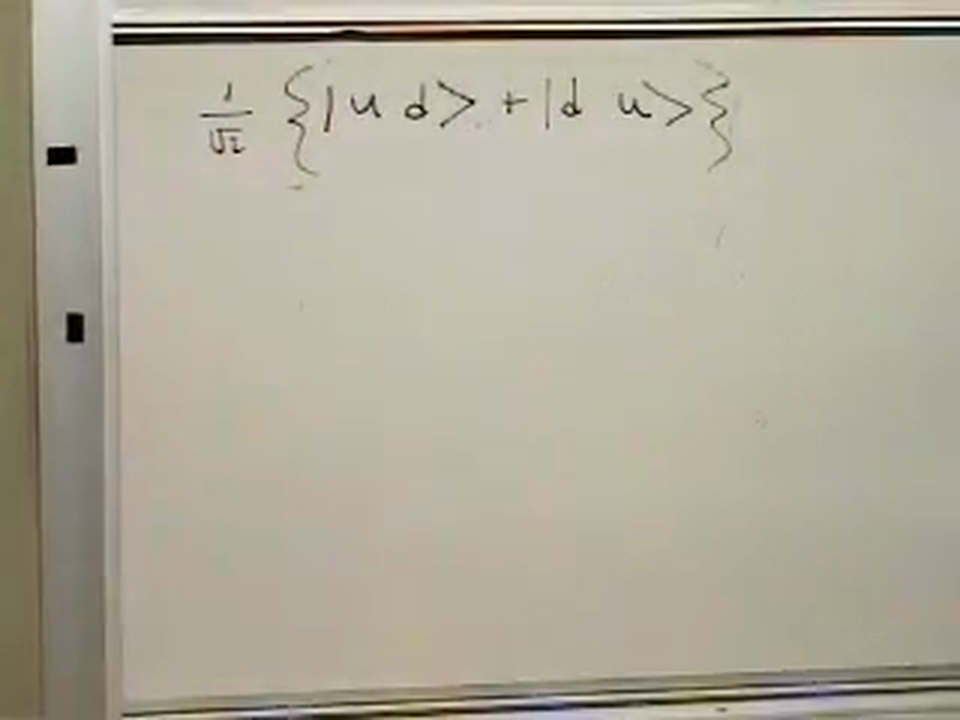
\includegraphics[width=0.82\linewidth]{lecture_04_figure_10.png}
\caption{最初のもつれ重ね合わせは1つの上向きと1つの下向きを含むが、どちらの結果も前もって粒子に割り当てない。}
\lectureframe{01:29:30}
\end{figure}

どちらの電子も単独でどのように見えるかを見るには、三つの局所期待値を計算する。第一成分については、
\begin{equation}
  \sigma_1\ket{\psi_+}
  =
  \frac{1}{\sqrt2}
  \left(\ket{dd}+\ket{uu}\right),
\end{equation}
であり、これは\(\ket{\psi_+}\)に直交する。したがって
\begin{equation}
  \bra{\psi_+}\sigma_1\ket{\psi_+}=0.
\end{equation}
同様に、
\begin{equation}
  \sigma_2\ket{\psi_+}
  =
  \frac{i}{\sqrt2}
  \left(\ket{dd}-\ket{uu}\right),
\end{equation}
なので
\begin{equation}
  \bra{\psi_+}\sigma_2\ket{\psi_+}=0.
\end{equation}
第三成分については、
\begin{equation}
  \sigma_3\ket{\psi_+}
  =
  \frac{1}{\sqrt2}
  \left(\ket{ud}-\ket{du}\right),
\end{equation}
であり、二つの対角寄与は相殺する：
\begin{equation}
  \bra{\psi_+}\sigma_3\ket{\psi_+}
  =\frac12(1-1)=0.
\end{equation}
したがって
\begin{equation}
  \begin{aligned}
    \bra{\psi_+}\sigma_i\ket{\psi_+}&=0,\\
    \bra{\psi_+}\tau_i\ket{\psi_+}&=0,
    \qquad i=1,2,3.
  \end{aligned}
  \label{eq:l04-zero-local-spin}
\end{equation}

\begin{figure}[htbp]
\centering
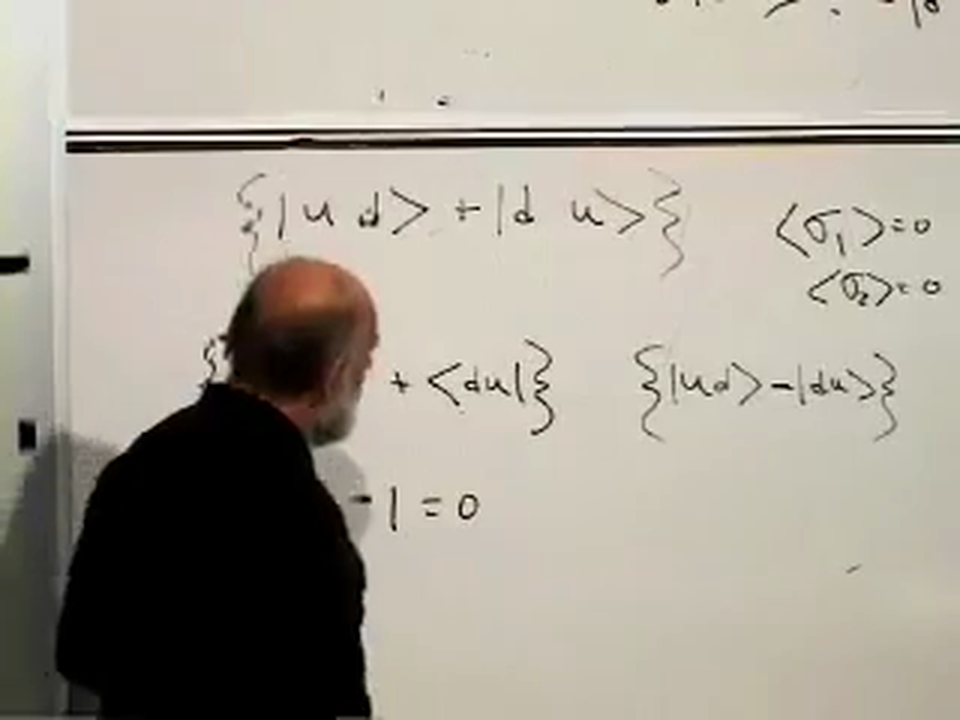
\includegraphics[width=0.84\linewidth]{lecture_04_figure_11.png}
\caption{変換された状態と相殺\(1-1=0\)は、局所スピン期待値が消えることを確立する。}
\lectureframe{01:35:50}
\end{figure}

任意の方向について、
\begin{equation}
  \bra{\psi_+}\sigma_{\hat n}\ket{\psi_+}=0,
  \qquad
  \bra{\psi_+}\tau_{\hat n}\ket{\psi_+}=0.
  \label{eq:l04-zero-arbitrary-local-spin}
\end{equation}
各局所測定の結果は\(\pm1\)のみであるから、期待値がゼロであることは
\begin{equation}
  P(\sigma_{\hat n}=+1)
  =
  P(\sigma_{\hat n}=-1)
  =
  \frac12,
\end{equation}
を意味し、第二の電子についても同様である。どの方向も、どちらの電子も単独では偏極させない。これは一スピン純粋状態では不可能であるが、もつれた純粋状態の一部にとっては完全に可能である。

\begin{classroomqa}
\lecturetimestamp{01:38:23}
\audiencequestion{半々の局所的な結果と、一方の電子を測定すれば他方について分かるという事実は、同じ主張なのか。}
\lecturerresponse{いいえ。まず電子\(2\)を無視する。電子\(1\)だけについて測定したどの方向でも、半々の分布が得られる。これにより、局所的な偏りが存在しないことが確立される。相関は、記録された二つの結果がどのように関係しているかについての、別個の結合的な主張である。もつれは両方の特徴を与えるが、一方をもう一方の証明の代用にしてはならない。}
\end{classroomqa}

\section{ベル以前の相関}

相関それ自体は、量子に固有のものではない。1セント硬貨と10セント硬貨を混ぜ、見ずに分けてから、一方を調べる。調べる前は、どちらの物体も1セント硬貨である確率が50パーセントであるが、ここで1セント硬貨が見つかれば、遠方の物体は10セント硬貨であるとわかる。どちらの部分も単独では確定した情報を持たなくても、その対は確定した情報を運んでいる。

\begin{classroomqa}
\lecturetimestamp{01:41:45}
\audiencequestion{1セント硬貨と10セント硬貨の推論は、元の対にそれぞれがちょうど1枚ずつ含まれているとわかっている場合にのみ成り立つのか。}
\lecturerresponse{そのとおりである。古典的な推論は、信頼できる準備に依存している。同様に、量子相関の予測は、2電子系が指定された結合状態に準備されている場合にのみ適用される。}
\end{classroomqa}

\begin{classroomqa}
\lecturetimestamp{01:42:09}
\audiencequestion{\(\ket{\psi_+}\)について、第3成分の測定が両方とも上である確率はゼロか。それは、あらゆる軸に沿ってスピンが逆向きであることを証明するのか。}
\lecturerresponse{第3軸基底における\(uu\)の確率はゼロであり、第3軸の2つの結果は逆向きである。しかし、第2の結論はこのプラス符号の状態には強すぎる。その局所スピンはあらゆる方向でゼロである一方、その結合相関は方向に依存する。普遍的に逆向きの結果は、講義の最後に導入されるマイナス符号の一重項状態に属する。}
\end{classroomqa}

\begin{classroomqa}
\lecturetimestamp{01:43:51}
\audiencequestion{古典的な対を、一方の面が常に他方の面と逆向きになるように溶接された二枚の硬貨として想像できるか。}
\lecturerresponse{それは、振ることが連結を乱さない限り、固定された反相関に対する可能な古典的機構である。それは準備の時点で確立された隠れた古典的配置にとどまる。この類推は意図的に暫定的なものであり、ベル定理は、そのような古典的説明がすべてどこで破綻するかを検証する。}
\end{classroomqa}

\begin{classroomqa}
\lecturetimestamp{01:44:32}
\audiencequestion{一方の結果がすでに相手の結果を決定しているなら、大数の法則はどこで関与するのか。}
\lecturerresponse{条件付きの確実性は、結合状態と一方の結果が与えられたときの、1回の試行についての主張である。約束された相関が信頼できることを実験的に検証し、期待値や不完全な確率を推定するには、依然として繰り返しの試行が必要である。大数の法則は、それらの繰り返しの頻度を理論的分布に結びつける。}
\end{classroomqa}

2人の観測者は、途方もない距離だけ離れているかもしれない。一方の結果を見ることは、局所的な観測者が他方の結果について知っていることを変えるが、遠方の観測者に制御可能なメッセージを送るわけではない。この段階では、状況は依然として分離された1セント硬貨と10セント硬貨に似ている。

\begin{classroomqa}
\lecturetimestamp{01:46:46}
\audiencequestion{分離された1セント硬貨と10セント硬貨の描像は、量子対を考える正しい方法なのか。}
\lecturerresponse{それは正しい最初の古典的比較ではあるが、最終的な量子論的説明ではない。ベルの定理は、あらかじめ存在する古典的性質を運ぶ対と、もつれた量子対との間の測定可能な違いに関するものである。その区別は、必要な相関が計算されるまで延期される。}
\end{classroomqa}

\section{一重項とその準備}

黒板での計算の最後で、プラス符号をマイナスに置き換える。
\begin{equation}
  \ket{\psi_-}
  =
  \frac{1}{\sqrt2}
  \left(\ket{ud}-\ket{du}\right).
  \label{eq:l04-singlet}
\end{equation}
この変更により、式~\eqref{eq:l04-zero-local-spin}の局所期待値はゼロに等しいままであり、第3軸の結果も逆向きのままである。一方、横方向の結合相関は変化する。このマイナス符号の状態がスピン一重項であり、2つのスピンがすべての共通測定軸に沿って逆向きになる回転不変な状態である。

\begin{figure}[htbp]
\centering
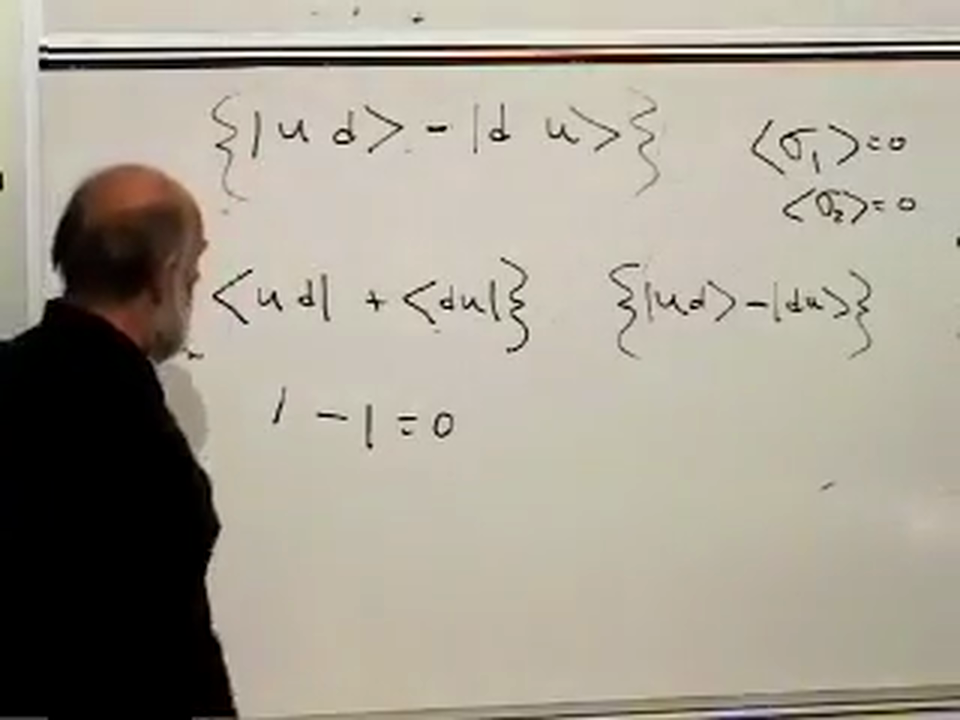
\includegraphics[width=0.84\linewidth]{lecture_04_figure_12.png}
\caption{黒板での最終的な変更は、対称な重ね合わせをマイナス符号の一重項に置き換えつつ、局所スピンをゼロに保つ。}
\lectureframe{01:47:25}
\end{figure}

ここで用いる単純化された物理的描像では、二つの局在した電子磁気モーメントを相互作用するのに十分近づけると、より高いエネルギーの配列が光子放出によって緩和する。優先的な外部軸がなければ、より低いスピン状態は回転対称な一重項で表される。正確な相互作用と、相対位相が負でなければならない理由には、さらなる計算が必要である。

\begin{classroomqa}
\lecturetimestamp{01:49:02}
\audiencequestion{実際の準備とは、単に二つの電子を近づけて待つだけなのでしょうか。}
\lecturerresponse{この理想化された模型では、そのとおりである。スピン-スピン相互作用を作用させ、輻射緩和によって低い状態へ落ち着かせればよい。電子は、その磁気相互作用が有効に働く程度に、十分近くに、十分長くあればよい。実際の準備プロトコルでは、軌道状態や競合する相互作用も制御しなければならない。}
\end{classroomqa}

\begin{classroomqa}
\lecturetimestamp{01:49:16}
\audiencequestion{これは単にパウリの排他原理ではないのでしょうか。}
\lecturerresponse{いいえ。二つの電子には区別可能な空間的位置が割り当てられているので、そのスピンについての議論では、重なり合う軌道波動関数を反対称化する必要はまだない。排他性が関係するのは、同一の電子が重なり合う一粒子状態を占めるときである。現在のもつれの議論は、離れたサイトに対してもすでに成り立っている。}
\end{classroomqa}

\begin{classroomqa}
\lecturetimestamp{01:50:31}
\audiencequestion{普通の電子ビームには、そのような相互作用する対が自然に含まれるのでしょうか。}
\lecturerresponse{通常は含まれない。ビームは希薄であり、典型的な電子は、利用可能な飛行時間の間に有意なスピン-スピン相互作用が働くには離れすぎている。衝突や意図的に閉じ込める相互作用によってもつれた対を作ることはできるが、同じビームに属しているというだけでは作られない。}
\end{classroomqa}

\begin{classroomqa}
\lecturetimestamp{01:51:45}
\audiencequestion{磁気相互作用にはどの程度の距離が必要なのでしょうか。}
\lecturerresponse{普遍的な鋭いカットオフは存在しない。決定的な量は相互作用の時間スケールである。この講義では、速い結合に対して\(10^{-11}\,\mathrm{cm}\)程度の粗い微視的見積もりを与えている。より大きな間隔では、エネルギー分裂は小さくなり、放出される光子はより長い波長をもち、緩和にはるかに長い時間がかかる。原理的には十分長く待てば補償できるが、普通のビームでは時間が足りなすぎる。}
\end{classroomqa}

\begin{classroomqa}
\lecturetimestamp{01:53:10}
\audiencequestion{なぜ一重項はプラス符号ではなくマイナス符号を含まなければならないのでしょうか。}
\lecturerresponse{それは局所的な半々の統計からは明らかではない。というのも、それらの統計は二つの相対位相に対して同一だからである。答えは、状態が回転の下でどのように変換するか、そして相互作用がどのように全スピンゼロを選び出すかにある。その導出は次回の講義に属する。}
\end{classroomqa}

講義は今や意図された閾値を越えた。単一の純粋なスピンは常に確定した上向き軸をもつ。純粋な対は、どちらの構成要素にも純粋状態を割り当てる必要はないが、それでもそれらの結果の間の厳密な関係を符号化することができる。その余分な構造がもつれである。ベルの定理は、なぜいかなる古典的な硬貨と硬貨の物語もそのすべてを再現できないのかを決定づけるであろう。
